\numberedsection{RF5.4 Borrar relación}

\subsection*{Descripción}
Permite a los usuarios eliminar una categoría existente en el sistema. La eliminación de una categoría solo será permitida si no está asociada a productos.\par
\vspace{0.15cm}

\textbf{Pre-condición}\par
El usuario debe tener la sesión iniciada en Mini PIM. La categoría a eliminar debe de existir en el sistema y no debe estar asociada a ningún producto.\par
\vspace{0.15cm}

\textbf{Post-condición}
\begin{itemize}
    \item Caso de éxito: La categoría es eliminada correctamente, se elimina de la lista de categorías y se actualiza la base de datos.
    \item Caso mínimo: El sistema notifica al usuario el resultado de la acción de borrar categoría: exitosa o fallida.
\end{itemize}

\textbf{Prioridad: }
Media
\vspace{0.15cm}

\textbf{Autor: }
Janine Bernadeth Olegario Laguit\par
\vspace{0.15cm}

\textbf{Control de cambios: } Versión 1: Definición del caso de uso

\numberedsubsection{Escenario principal}
\begin{enumerate}
    \item El usuario accede a la sección de gestión de categorías.
    \item El sistema muestra la lista de categorías existentes.
    \item El usuario selecciona la opción de \enquote{Eliminar} una categoría.
    \item El sistema muestra una ventana emergente de confirmación para la eliminación de la categoría.
    \item El sistema verifica si la categoría está asociada a algún producto.
    \item Si la categoría no está asociada algún producto, el usuario confirma la eliminación.
    \item El sistema elimina la categoría de la base de datos.
    \item El sistema actualiza la lista de categorías, eliminando la categoría seleccionada.
    \item El sistema muestra un mensaje de éxito indicando que la categoría ha sido eliminada correctamente.
\end{enumerate}

\numberedsubsection{Escenarios alternativos}
\begin{description}
  
    \item[4.a] El usuario cancela la acción de eliminar la categoría seleccionada.
    \begin{enumerate}
        \item[4.a.1] El sistema regresa a la sección de gestión de categorías sin realizar ningún cambio.
    \end{enumerate}

     \item[6.a] La categoría seleccionada no puede ser eliminada por estar asociada a productos.
    \begin{enumerate}
        \item[6.a.1] El sistema muestra un mensaje de error indicando que no se puede eliminar la categoría debido a que está asociada a algún producto.
        \item[6.a.2] El sistema regresa a la sección de gestión de categorías.
    \end{enumerate}
\end{description}

\numberedsubsection{Casos de Prueba}
\underline{Escenario: Principal}\par
\vspace{0.15cm}

\textbf{Dado} que he iniciado sesión con mi cuenta de usuario correspondiente,\par
\textbf{Y} estoy en el apartado de Categorías,\par
\textbf{Cuando} selecciono la opción de \enquote{Eliminar} en una categoría,\par
\textbf{Y} confirmo la eliminación de la categoría en la ventana emergente,\par
\textbf{Entonces} el sistema elimina la categoría de la base de datos,\par
\textbf{Y} actualiza la lista de categorías, removiendo la categoría eliminada,\par
\textbf{Y} muestra un mensaje de éxito indicando que la categoría ha sido eliminada correctamente.\par

\vspace{0.20cm}

\underline{Escenario: Alternativo 4.a}\par
\vspace{0.15cm}

\textbf{Dado} que he iniciado sesión con mi cuenta de usuario correspondiente,
\textbf{Y} estoy en el apartado de Categorías,\par
\textbf{Cuando} selecciono la opción de \enquote{Eliminar} en una categoría,\par
\textbf{Y} selecciono la opción de \enquote{cancelar} en la ventana emergente de confirmación,\par
\textbf{Entonces} el sistema regresa a la sección de gestión de categorías,\par
\textbf{Y} muestra la lista de categorías sin realizar ningún cambio.\par


\vspace{0.20cm}

\underline{Escenario: Alternativo 6.a}\par
\vspace{0.15cm}

\textbf{Dado} que he iniciado sesión con mi cuenta de usuario correspondiente,\par
\textbf{Y} estoy en el apartado de Categorías,\par
\textbf{Cuando} selecciono la opción de \enquote{Eliminar} en una categoría,\par
\textbf{Y} la categoría esta asociada algún producto,\par
\textbf{Y} el sistema detecta que la categoría está asociada a algún producto,\par
\textbf{Entonces} el sistema muestra un mensaje de error indicando que no se puede eliminar la categoría,\par
\textbf{Y} el sistema me redirige a la sección de gestión de categorías.\par


\vspace{0.20cm}

\numberedsubsection{Bocetos}
\begin{figure}[H]
    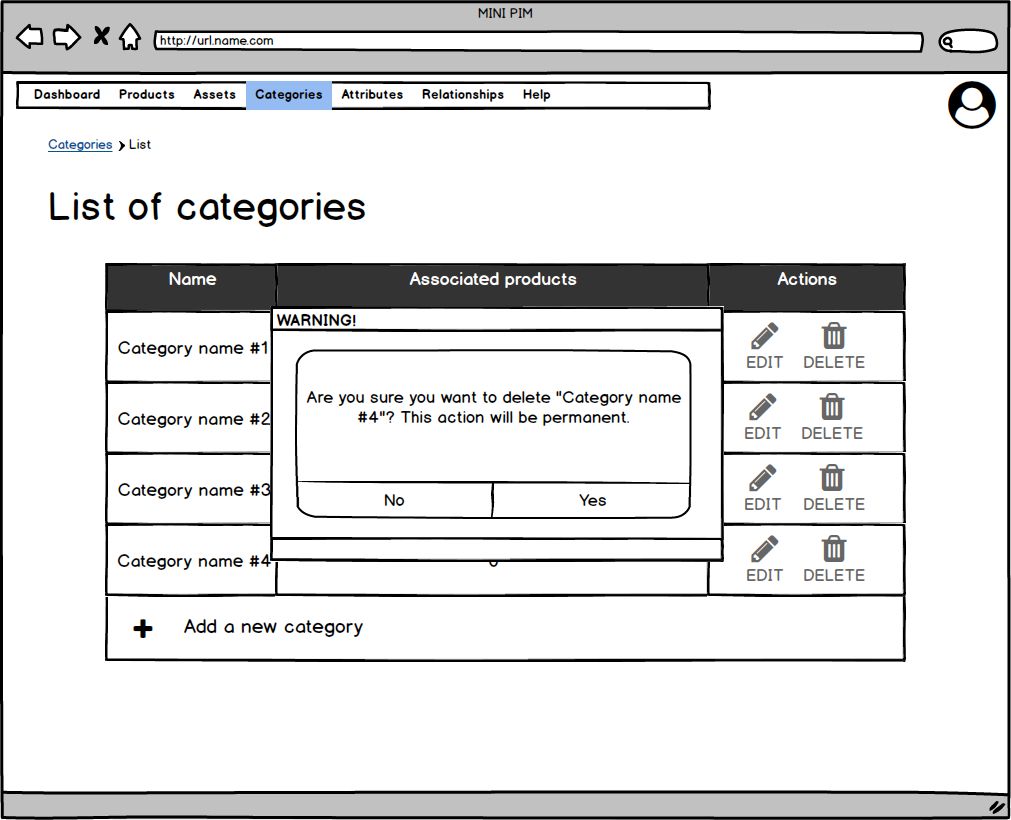
\includegraphics[width=1\linewidth]{mockups/RF4.4_1.png}
    \caption{Mensaje esperando confirmación para eliminar categoría}
   \end{figure}
\vspace{1.0cm}

\begin{figure}[H]
    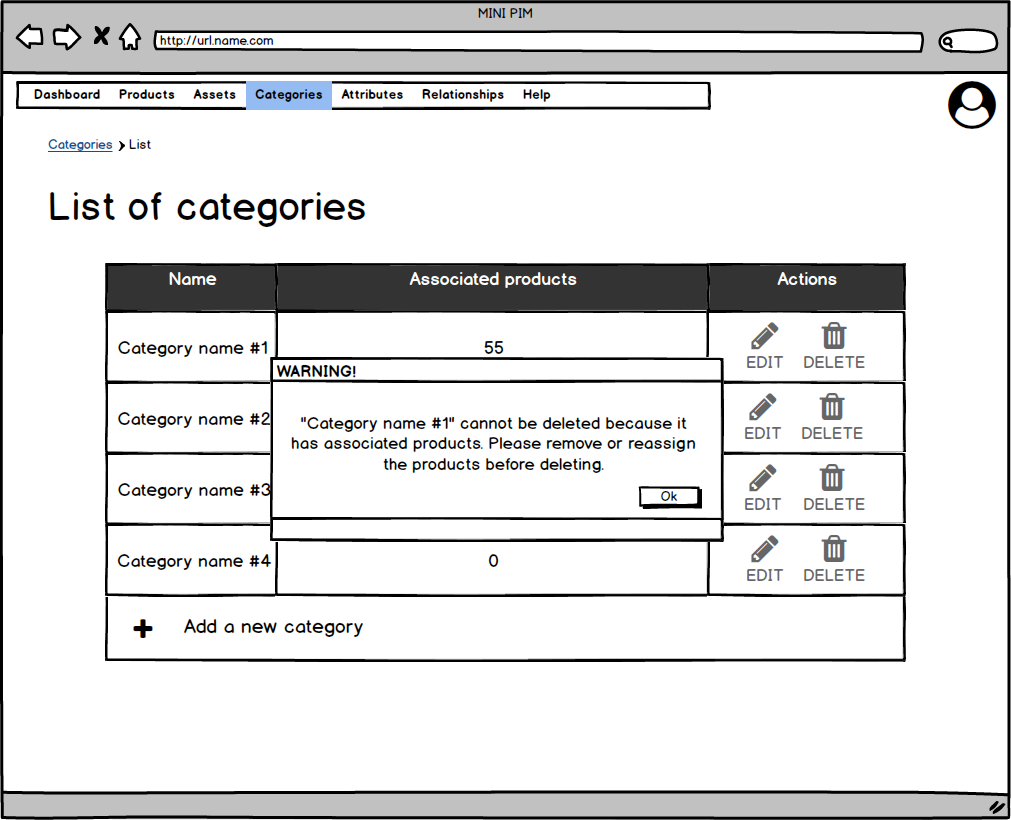
\includegraphics[width=1\linewidth]{mockups/RF4.4_2.png}
    \caption{Mensaje de error porque la categoría a borrar tiene productos asociados}
   \end{figure}
\vspace{1.0cm}

\newpage %Inicia en una nueva página otro caso de uso